\chapter{Der Simulator}

\section{Die grafische Benutzerschnittstelle}

Die grafische Benutzerschnittstelle (GUI; Graphical User Interface) pr\"{a}sentiert sich standardm\"{a}�ig wie in Abbildung \ref{fig:StandardGUI}.

\begin{figure}[htbp]
	\centering
	\fbox{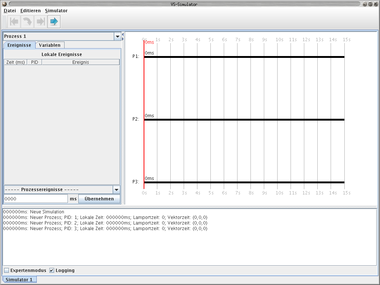
\includegraphics{images/ss-neue-simulation-klein}}
	\caption{Standard GUI}
	\label{fig:StandardGUI}
\end{figure}

Im folgenden werden in die einzelnen Komponenten des GUIs eingegangen.

\subsection{Die Men\"{u}zeile}

Im Datei-Men\"{u} (Abbildung \ref{fig:DateiMenue}) lassen sich neue Simulationen erstellen oder die aktuell ge\"{o}ffnete Simulation schliessen. Neue Simulationen \"{o}ffnen sich standardm\"{a}�ig in einem neuen Tab. Es k\"{o}nnen allerdings auch neue Simulationsfenster, die wiederrum eigene Tabs besitzen, ge\"{o}ffnet oder geschlossen werden. In jedem Tab befindet sich eine von den Anderen vollst\"{a}ndig unabh\"{a}ngige Simulation. Es k\"{o}nnen somit beliebig viele Simulationen parallel ausgef\"{u}hrt werden. Die Men\"{u}eintr\"{a}ge ``\"{O}ffnen'', ``Speichern'' und ``Speichern unter'' dienen f\"{u}r das Laden und Speichern von Simulationen. 

\begin{figure}[htbp]
	\centering
	\fbox{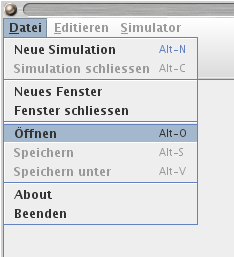
\includegraphics[width=14cm]{images/ss-datei-menu}}
	\caption{``Datei''-Men\"{u}}
	\label{fig:DateiMenue}
\end{figure}

\"{U}ber das ``Editieren''-Men\"{u} gelangt man zu den Simulationseinstellungen. Es werden auch alle beteiligten Prozesse zum Editieren aufgelistet. Und das Men\"{u} ``Simulator'' bietet die selben Optionen wie die Toolbar (s.u.).

\subsection{Die Toolbar}

Oben links befindet sich die Toolbar (Abbildung \ref{fig:Toolbar}) des Simulators. Die Toolbar enth\"{a}lt die Funktionen, die vom Benutzer am schnellsten und h\"{a}ufigsten verwendet werden.

Die Toolbar bietet vier verschiedene Aktionen an:

\begin{itemize}
	%\setlength{\itemsep}{-1mm}
	\item Starten der Simulation, kann nur bet\"{a}tigt werden, wenn die Simulation derzeit nicht l\"{a}uft.
	\item Pausieren der Simulation, kann nur bet\"{a}tigt werden, wenn die Simulation derzeit l\"{a}uft.
	\item Wiederholen der Simulation, kann nicht bet\"{a}tigt werden, wenn die Simulation noch nicht gestartet wurde.
	\item Zur\"{u}cksetzen der Simulation, kann nur bet\"{a}tigt werden, wenn die Simulation pausiert wurde oder wenn die Simulation abgelaufen ist.
\end{itemize}

\begin{figure}[htbp]
	\centering
	\fbox{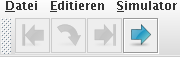
\includegraphics[width=5cm]{images/ss-neue-simulation-toolbar}}
	\caption{Die Men\"{u}zeile inklusive Toolbar}
	\label{fig:Toolbar}
\end{figure}


Die Toolbar l\"{a}sst sich auch nach Belieben repositionieren (z.B. links, rechts oder unten des Simulatorfensters). Hierf\"{u}r muss per ``Drag-n-Drop'' die ``raue Fl\"{a}che'' zur Zielposition gezogen werden.


\subsection{Die Visualisierung}

\begin{figure}[htbp]
	\centering
	\fbox{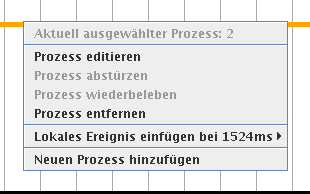
\includegraphics[width=8.8cm]{images/ss-rechtsklick-prozessbalken}}
	\caption{Rechtsklick auf einen Prozessbalken}
	\label{fig:RechtsklickProzessbalken}
\end{figure}

Mittig rechts (Abbildung \ref{fig:StandardGUI}) befindet sich die grafische Repr\"{a}sentation der Simulation. Die X-Achse repr\"{a}sentiert die Zeit in Millisekunden. Die aktuelle Simulation endet nach genau 15 Sekunden. In Abbildung \ref{fig:Visualisierung} sind 3 Prozesse (mit den PIDs 1, 2 und 3) dargestellt, die jeweils einen eigenen horizontalen schwarzen Balken besitzen. Auf diesen Prozessbalken kann man die jeweilige lokale Prozesszeit ablesen. Die vertikale rote Linie stellt die globale Zeit dar. 


Die Prozessbalken dienen auch f\"{u}r Start- und Zielpunkte von Nachrichten. Wenn beispielsweise Prozess 1 eine Nachricht zum Prozess 2 verschickt, so wird eine Linie vom einen Prozessbalken zum Anderen gezeichnet. Nachrichten, die ein Prozess an sich selbst schickt, werden nicht visualisiert.

Mit einem Linksklick auf einen Prozessbalken ist es ebenso m\"{o}glich einen Prozess zu editieren. Dies muss also nicht zwingend \"{u}ber das ``Simulator''-Men\"{u} geschehen. Ein Rechtsklick hingegen \"{o}ffnet ein Popup-Fenster mit weiteren Auswahlm\"{o}glichkeiten (Abbildung \ref{fig:RechtsklickProzessbalken}). Ein Prozess kann \"{u}ber das Popup-Men\"{u} nur dann abst\"{u}rzen oder wiederbelebt werden, wenn die Simulation aktuell l\"{a}uft.

\begin{figure}[htbp]
	\centering
	\fbox{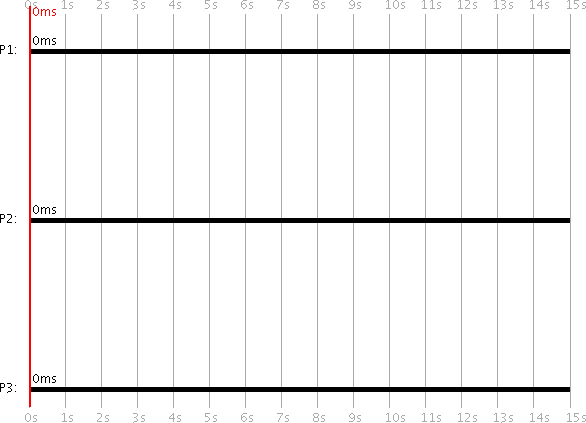
\includegraphics[width=14cm]{images/ss-visualisierung}}
	\caption{Visualisierung einer noch nicht gestarteten Simulation}
	\label{fig:Visualisierung}
\end{figure}


Generell kann die Anzahl der Prozesse nach belieben variieren. Die Dauer der Simulation betr\"{a}gt mindestens 5 -und maximal 120 Sekunden. Die Simulation endet erst, wenn die globale Zeit 15 Sekunden erreicht hat, und nicht, wenn eine lokale Prozesszeit die 15 Sekunden erreicht.

\subsection{Die Sidebar}

Mithilfe der Sidebar (mittig links, Abbildung \ref{fig:StandardGUI}) lassen sich Ereignisse bestimmter Prozesse verwalten. Ganz oben (Abbildung \ref{fig:Sidebar}) ist der zu verwaltende Prozess selektiert. Dort gibt es auch die Auswahl ``Alle Prozesse'', womit die Ereignisse aller Prozesse gleichzeitig verwaltet werden k\"{o}nnen. Unter ``Lokale Ereignisse'' versteht man die Ereignisse, die auftreten, wenn die zum jeweiligen Prozess lokale Prozesszeit eingetreten ist. Die darunterliegende Ereignistabelle listet alle programmierten Ereignisse (hier noch keine vorhanden) mitsamt Eintrittszeit sowie PID auf.

\begin{figure}[htbp]
	\centering
	\fbox{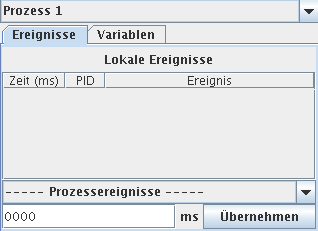
\includegraphics[width=9cm]{images/ss-sidebar}}
	\caption{Die Sidebar}
	\label{fig:Sidebar}
\end{figure}

F\"{u}r die Erstellung eines neuen Ereignisses kann man entweder mit Rechtsklick auf einen Prozessbalken (Abbildung \ref{fig:RechtsklickProzessbalken}) klicken, oder unterhalb der Ereignistabelle ein Ereignis ausw\"{a}hlen (Abbildung \ref{fig:Ereignisauswahl}), im Textfeld die Zeit eintragen und auf ``\"{U}bernehmen'' klicken.

\begin{figure}[htbp]
	\centering
	\fbox{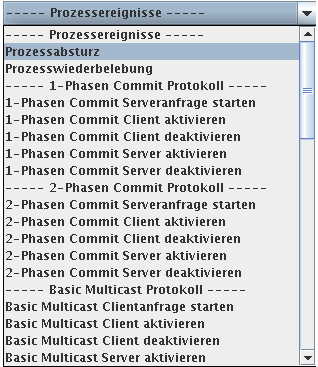
\includegraphics[width=9cm]{images/ss-ereignisauswahl}}
	\caption{Die Ereignisauswahl via Sidebar}
	\label{fig:Ereignisauswahl}
\end{figure}

Neben dem ``Ereignis''-Tab gibt es in der Sidebar einen Tab mit dem Namen ``Variablen''. Dort kann man alle Variablen des aktuell ausgew\"{a}hlten Prozesses editieren. Mehr dazu aber sp\"{a}ter. 

\subsection{Loggfenster}

\subsection{Expertenmodus}

\subsubsection{Lamport- und Vektorzeit}

\subsubsection{Loggfilter}

\subsubsection{Lokale und globale Ereignisse}

\section{Ereignisse}

\subsection{Prozessabsturz}

\subsection{Prozesswiederbelebung}

\subsection{Aktivierung und Deaktivierung von Protokollen}

\subsection{Weitere Protokollereignisse}

\section{Protokolle}

\subsection{Beispiel (Dummy) Protokoll}

\subsection{Das Ping-Pong Protokoll}

\subsection{Das Broadcast-Sturm Protokoll}

\subsection{Das Protokoll zur internen Synchronisierung in einem synchronen System}

\subsection{Christians Methode zur externen Synchronisierung}

\subsection{Berkeley Algorithmus zur internen Synchronisation}

\subsection{Das Ein-Phasen Commit Protokoll}

\subsection{Das Zwei-Phasen Commit Protokoll}

\subsection{Der ungen\"{u}gende (Basic) Multicast}

\subsection{Der zuverl\"{a}ssige (Reliable) Multicast}

\section{Zeitformate}

\subsection{``Normale Zeit''}

\subsection{Die Logische Uhr von Lamport}

\subsection{Die Vektor-Zeitstempel}

\section{Einstellungen}

\subsection{Simulationseinstellungen}

\subsection{Prozesseinstellungen}

\subsection{Protokolleinstellungen}

TODO: Farben der Prozessbalken, Farben der Nachrichten
